\chapter{Silizium-PVD}
\label{appendix:silicon}

\section{Voruntersuchungen}

\begin{figure}[h]
  \centering
  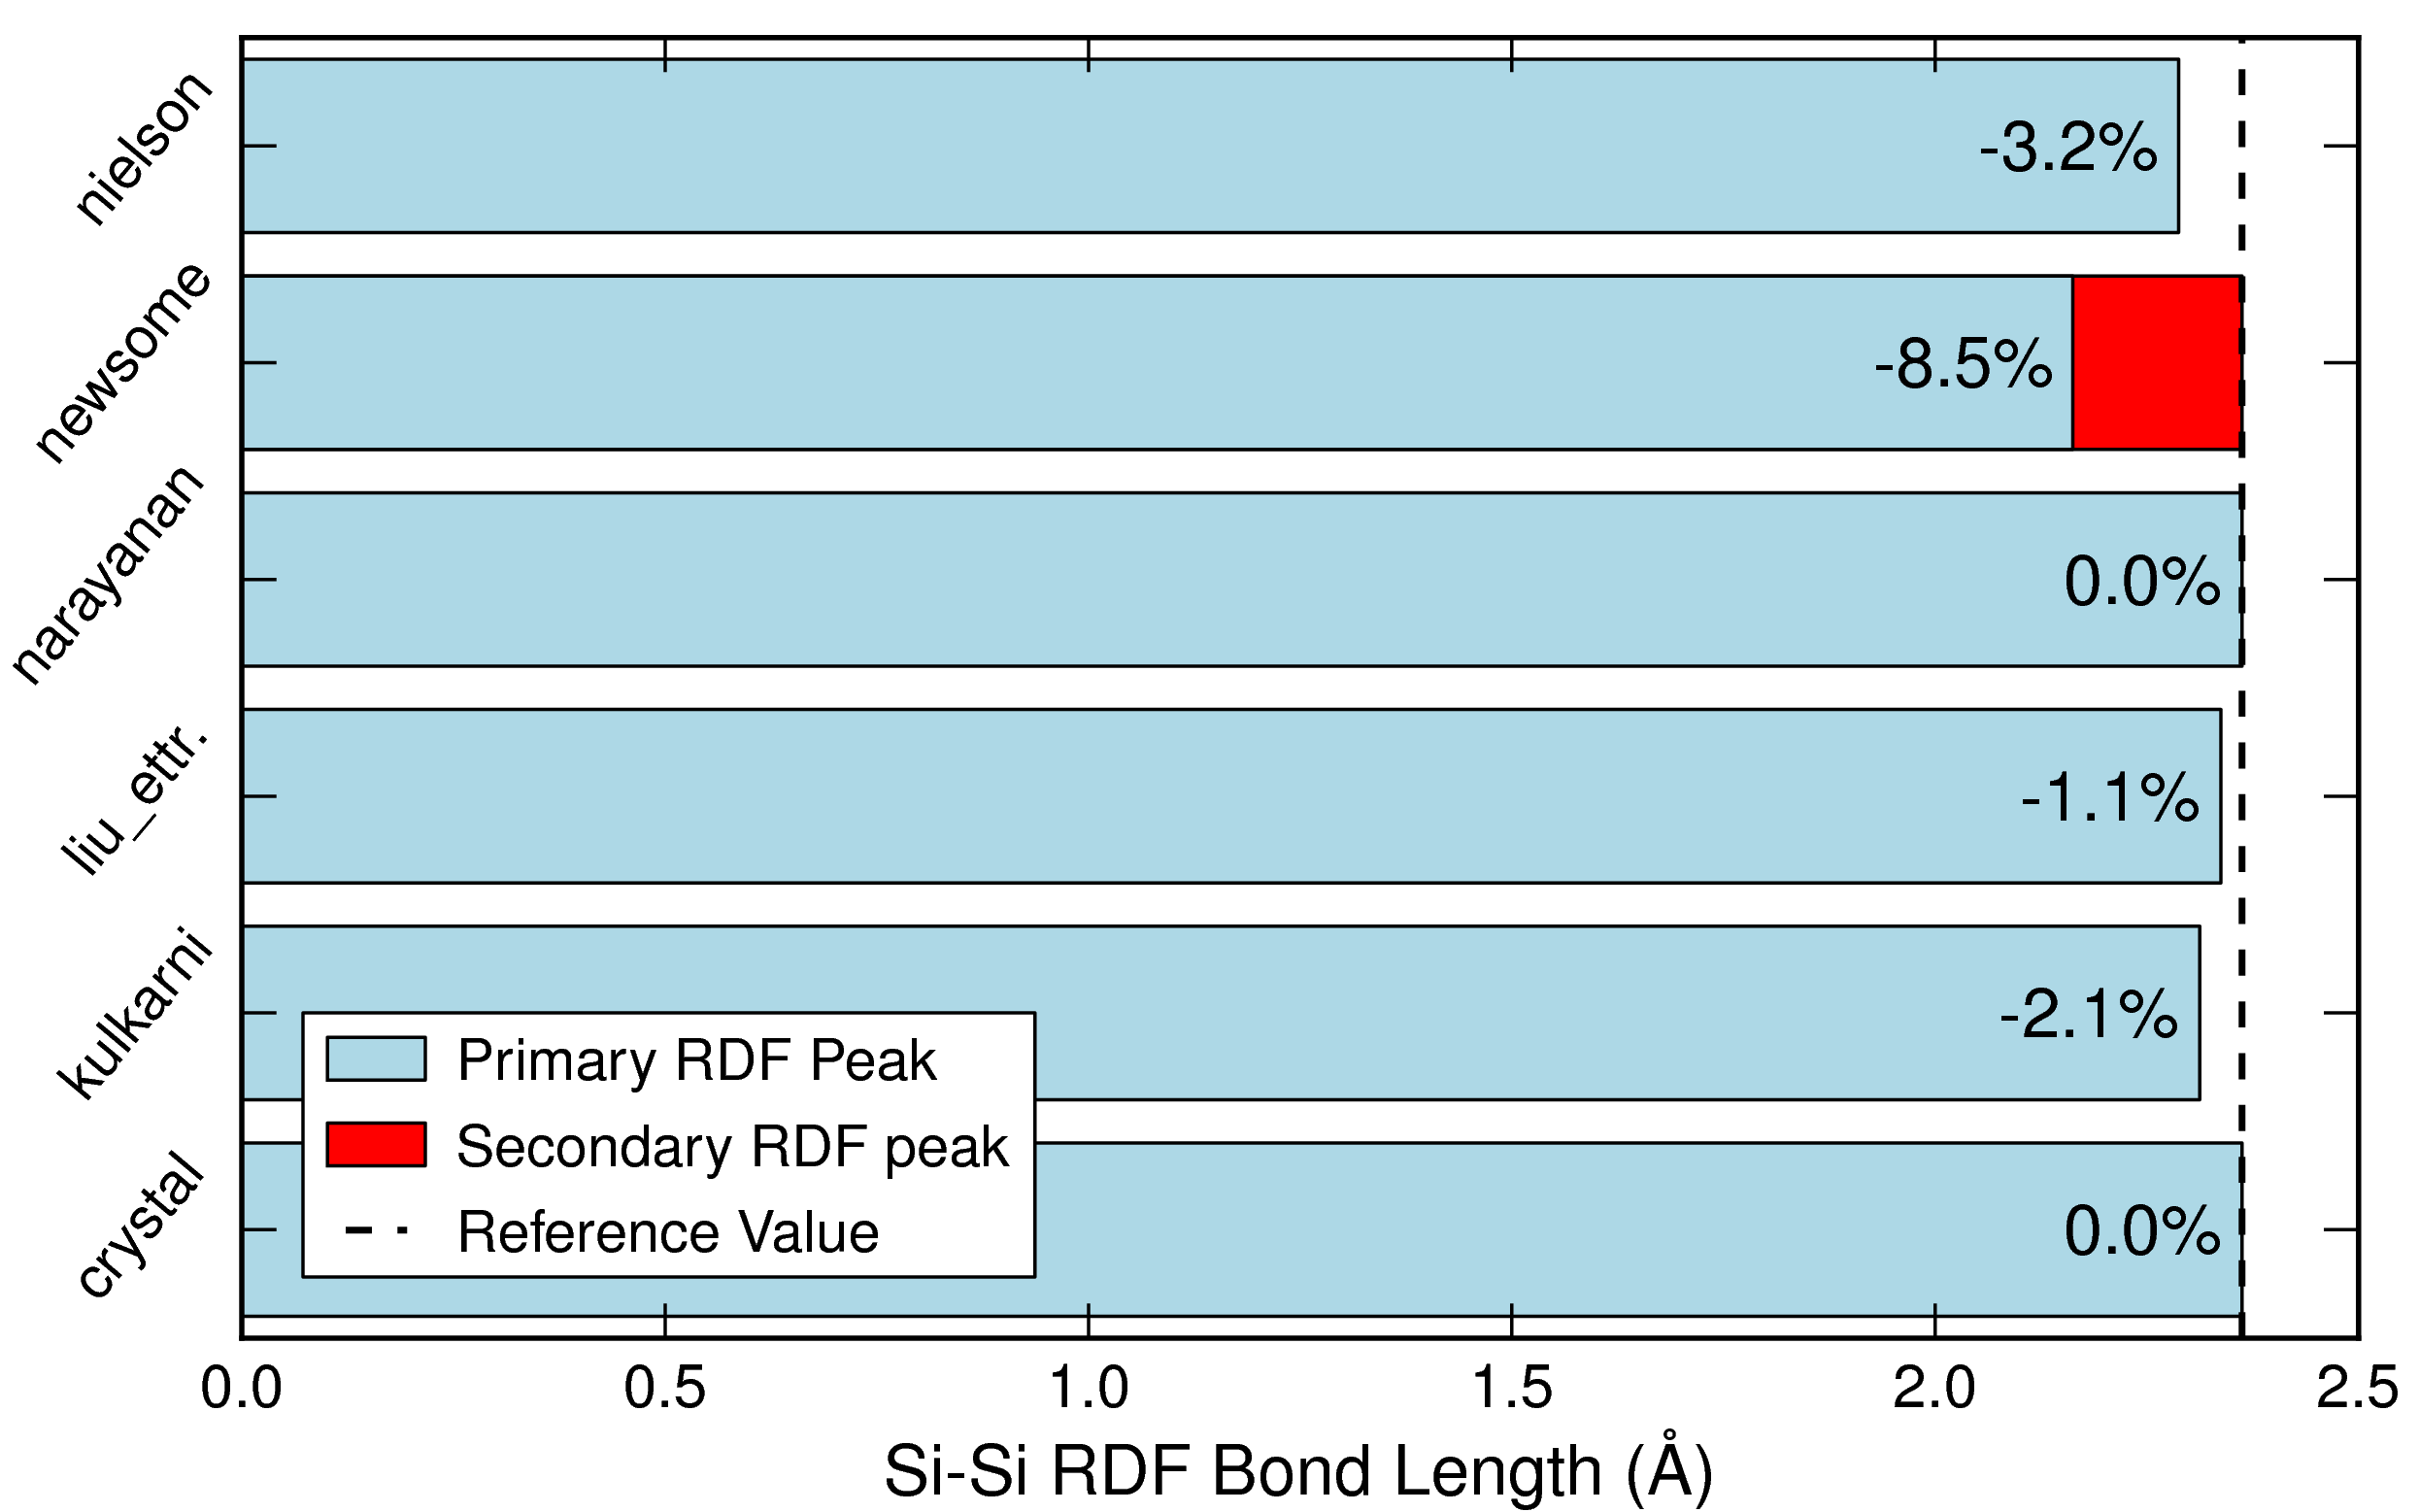
\includegraphics[width=10cm]{SiSi_npt_bondlengths}
  \caption[Bindungslängen von Kupfer im relaxierten Kristall für verschiedene Parametersätze]{Bindungslängen von Kupfer im relaxierten Kristall für verschiedene Parametersätze}
  \label{fig:sisibondlengths}
\end{figure}

\begin{figure}[h]
  \centering
  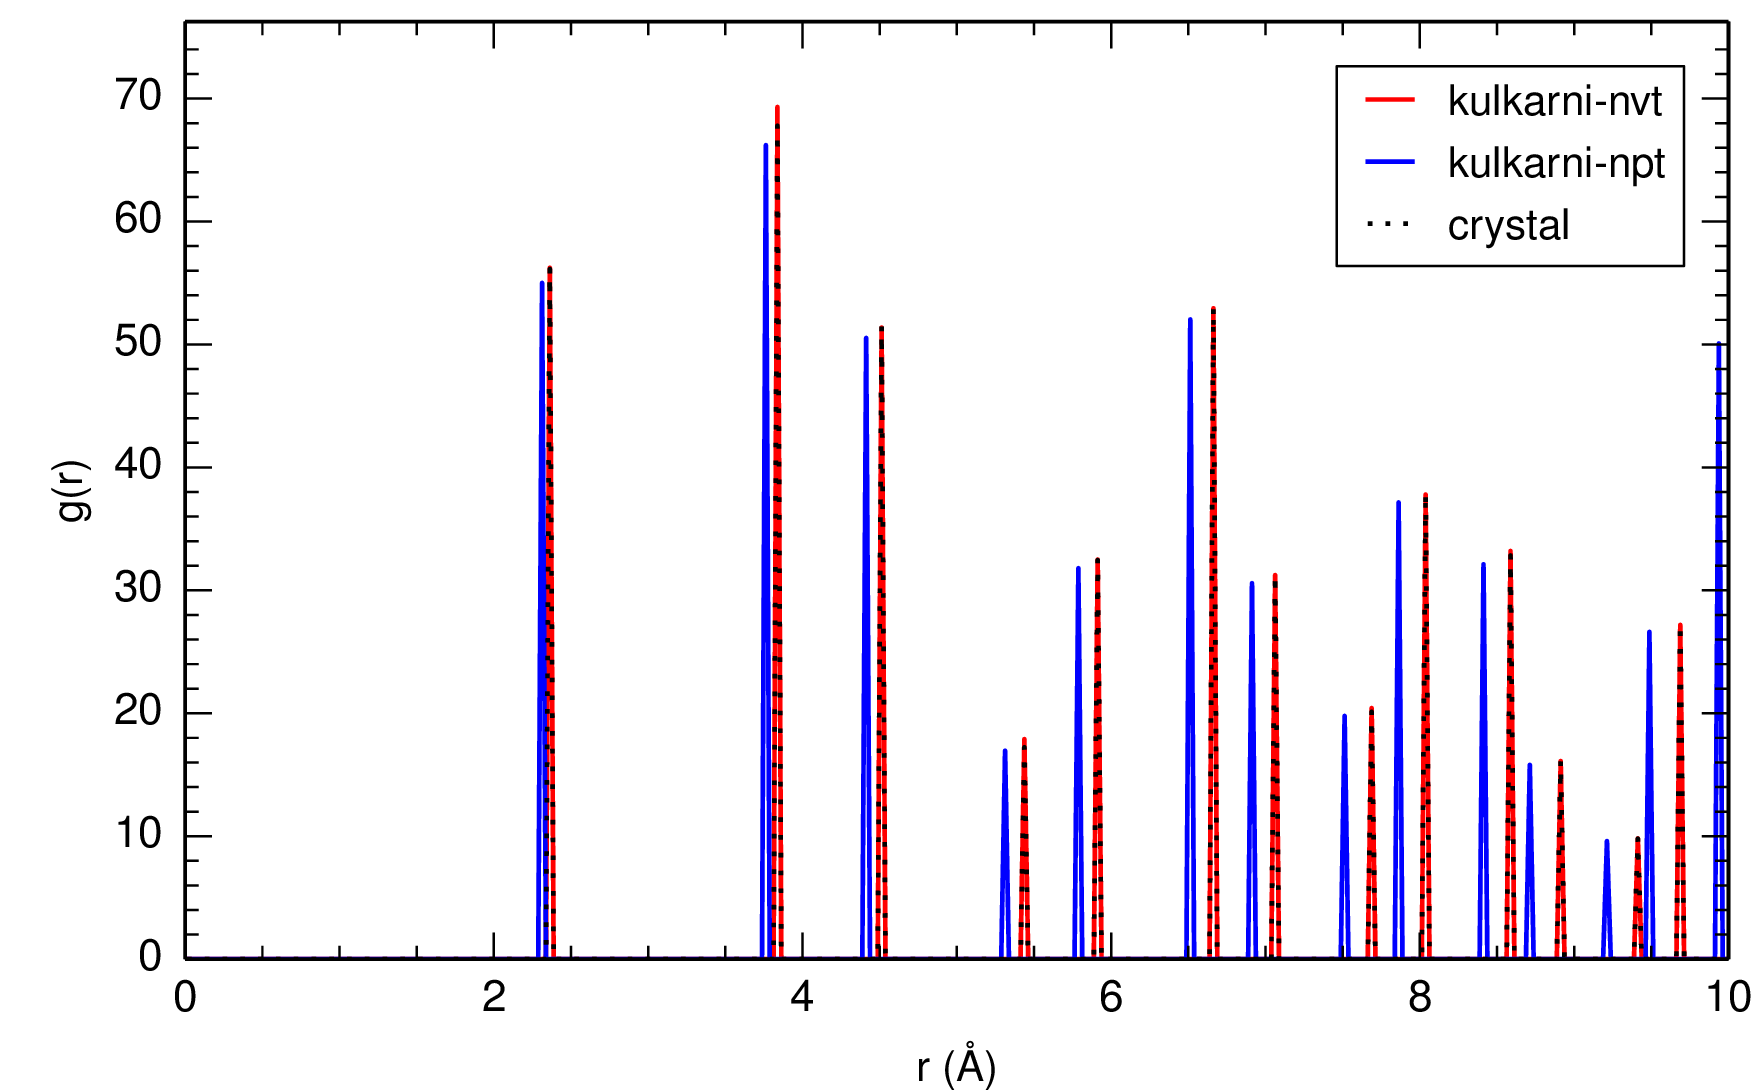
\includegraphics[width=10cm]{kulkarni_rdf_crystal}
  \caption[Radiale Verteilungsfunktion von kristallinem Silizium nach Relaxation mit Kulkarni-Parametersatz]{Radiale Verteilungsfunktion von kristallinem Silizium nach Relaxation mit Kulkarni-Parametersatz}
  \label{fig:kulkarnirdf}
\end{figure}

\begin{figure}[h]
  \centering
  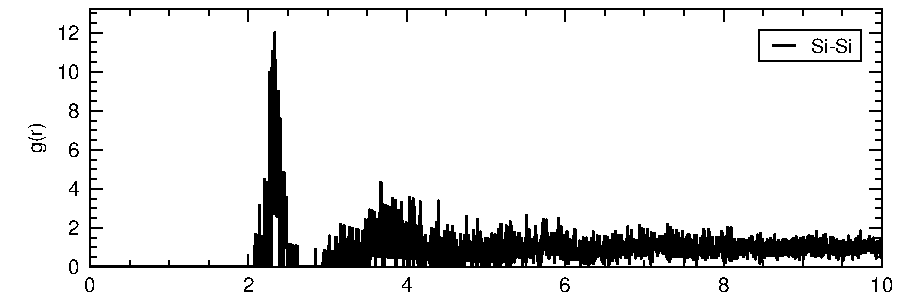
\includegraphics[width=\textwidth]{kulkarni_rdf_amorphous}
  \caption[Radiale Verteilungsfunktion von amorphem Silizium nach Relaxation mit Kulkarni-Parametersatz]{Radiale Verteilungsfunktion von amorphem Silizium nach Relaxation mit Kulkarni-Parametersatz}
  \label{fig:amorphousrdf}
\end{figure}

\begin{table}
  \begin{threeparttable}

    \caption[Vergleich der Eigenschaften amorpher Silizium-Materialien]{Vergleich der Eigenschaften amorpher Silizium-Materialien}
    \label{tab:amorphoussilicon}

    \oddrowcolors
    \begin{tabularx}{\textwidth}{|llXXlX|}
      \hline
      \textbf{Parametrisierung} & \multicolumn{2}{l}{\textbf{Bindungslänge}} & \textbf{Koord.} & \textbf{Dichte} & ~  \\
      \hline
      (kristallin) & \SI{2.352}{\angstrom} & ~                    & \num{4.00}  & \SI{2.330}{\gpcc} & ~                         \\
      (amorph)     & ~                     & ~                    & ~           & \SI{2.3}{\gpcc}   & \cite{remes_optical_1998} \\
      Al\_Al0\_AlN & \SI{2.379}{\angstrom} & \SI{+1.15}{\percent} & \num{4.59}  & \SI{2.373}{\gpcc} & \SI{+3.15}{\percent}      \\
      kulkarni     & \SI{2.339}{\angstrom} & \SI{-0.55}{\percent} & \num{4.05}  & \SI{2.361}{\gpcc} & \SI{+2.65}{\percent}      \\
      liu\_ettr.   & \SI{2.401}{\angstrom} & \SI{+2.08}{\percent} & \num{4.10}  & \SI{2.314}{\gpcc} & \SI{+0.61}{\percent}      \\
      narayanan    & \SI{2.383}{\angstrom} & \SI{+1.32}{\percent} & \num{4.05}  & \SI{2.365}{\gpcc} & \SI{+2.83}{\percent}      \\
      newsome      & \SI{2.153}{\angstrom} & \SI{-8.46}{\percent} & \num{1.17}  & \SI{2.398}{\gpcc} & \SI{+4.26}{\percent}      \\
      nielson      & \SI{2.411}{\angstrom} & \SI{+2.51}{\percent} & \num{4.82}  & \SI{2.358}{\gpcc} & \SI{+2.52}{\percent}      \\
      zhang        & \SI{2.357}{\angstrom} & \SI{+0.21}{\percent} & \num{4.39}  & \SI{2.329}{\gpcc} & \SI{+1.26}{\percent}      \\
      \hline
    \end{tabularx}

  \end{threeparttable}
\end{table}

\clearpage
\section{Precursorsimulationen}

\begin{figure}[h]

  \captionsetup[subfigure]{singlelinecheck=false}
  \def\subfigwidth{0.32\textwidth}
  \begin{subfigure}[t]{3.5cm}
    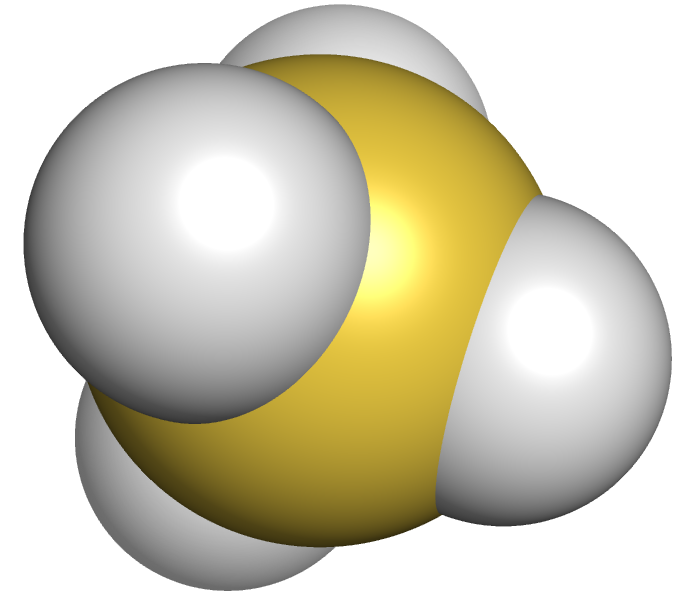
\includegraphics[width=\textwidth]{silane_nielson_stable}
    \subcaption{nielson: stabil}
  \end{subfigure}
  \hfill
  \begin{subfigure}[t]{4.5cm}
    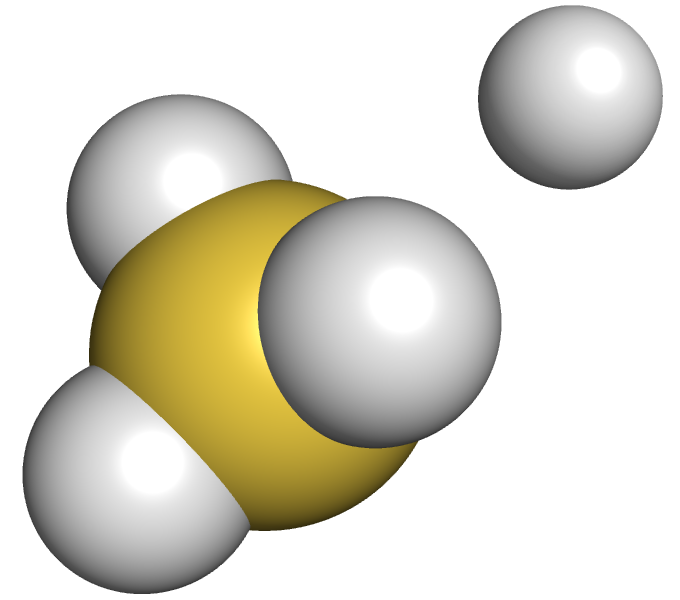
\includegraphics[width=\textwidth]{silane_narayanan_unstable}
    \subcaption{narayanan: instabil}
  \end{subfigure}
  \hfill
  \begin{subfigure}[t]{5cm}
    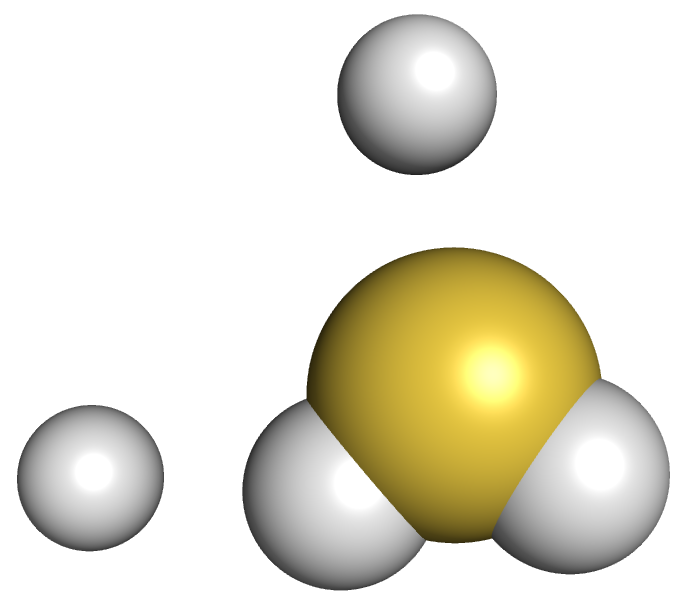
\includegraphics[width=\textwidth]{silane_liu_unstable}
    \subcaption{liu-ettringite: instabil}
  \end{subfigure}

  \caption[Stabilität von Silan]{Stabilitätsuntersuchungen von Silan bei 600K (\ce{SiH4}, Abscheidungstemperatur)}
  \label{fig:silanestability}

\end{figure}

\begin{figure}[h]

  \captionsetup[subfigure]{singlelinecheck=false}
  \def\subfigwidth{0.32\textwidth}
  \begin{subfigure}[t]{3cm}
    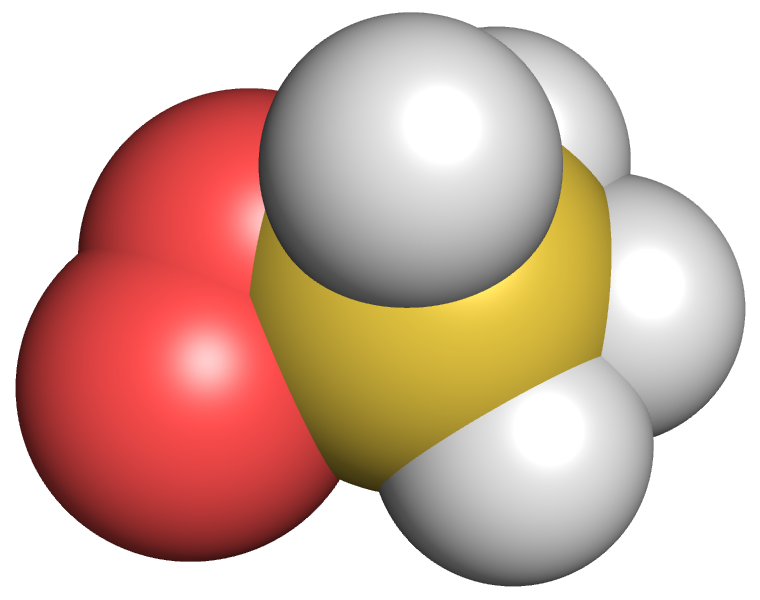
\includegraphics[width=\textwidth]{silane_reaction_zhang}
    \subcaption{zhang: Überzahl an Bindungen}
  \end{subfigure}
  \hfill
  \begin{subfigure}[t]{5cm}
    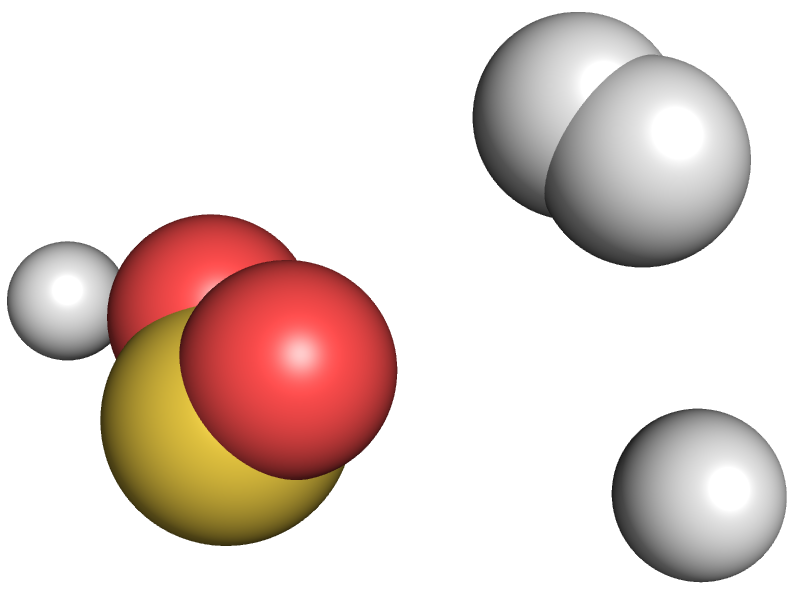
\includegraphics[width=\textwidth]{silane_reaction_newsome}
    \subcaption{newsome: stöchiometrisch perfekter Ausgang}
  \end{subfigure}
  \hfill
  \begin{subfigure}[t]{4.5cm}
    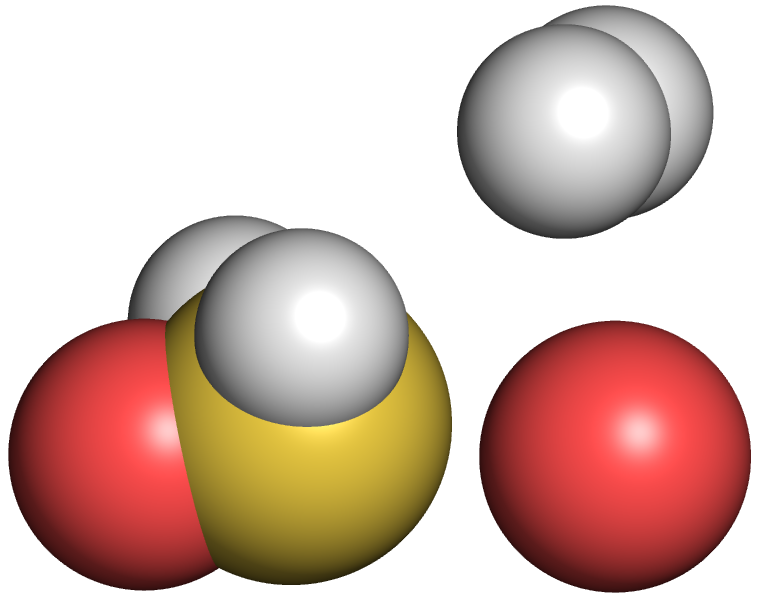
\includegraphics[width=\textwidth]{silane_reaction_kulkarni}
    \subcaption{kulkarni: Korrekte Bindungszahl, aber freier Sauerstoff}
  \end{subfigure}


  \caption[Reaktionen von Precursormolekülen]{Reaktionen einzelner Precursormoleküle}
  \label{fig:precursorreactions}

\end{figure}

\begin{figure}[h]

  \captionsetup[subfigure]{singlelinecheck=false}
  \begin{subfigure}[t]{4cm}
    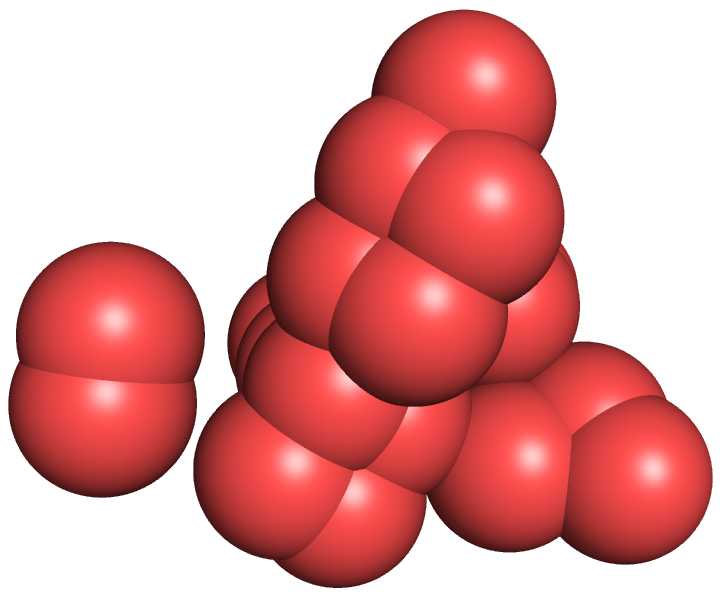
\includegraphics[width=\textwidth]{oxygen_cluster}
    \subcaption{kulkarni: \ce{O2}-Cluster}
  \end{subfigure}
  \hfill
  \begin{subfigure}[t]{5.5cm}
    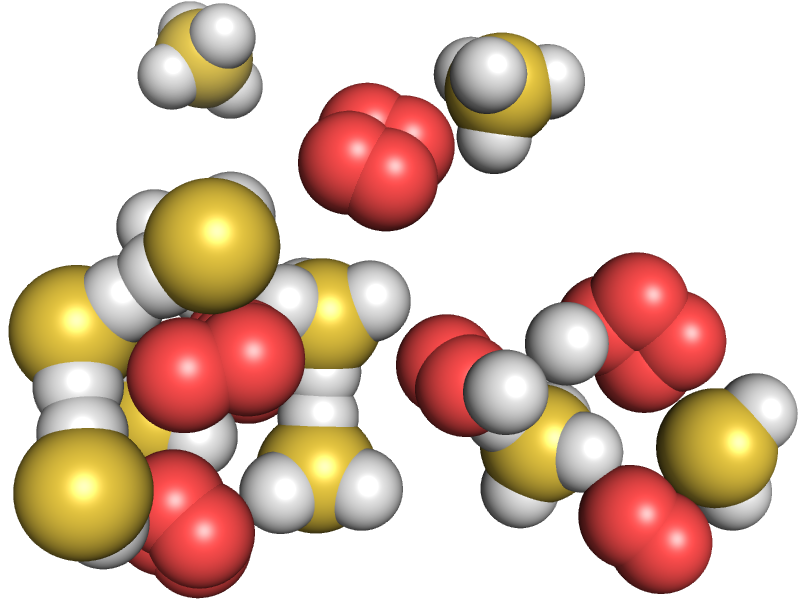
\includegraphics[width=\textwidth]{kulkarni_precursor_cluster}
    \subcaption{kulkarni: Cluster von Precursor-Molekülen}
  \end{subfigure}
  \hfill
  \begin{subfigure}[t]{4.5cm}
    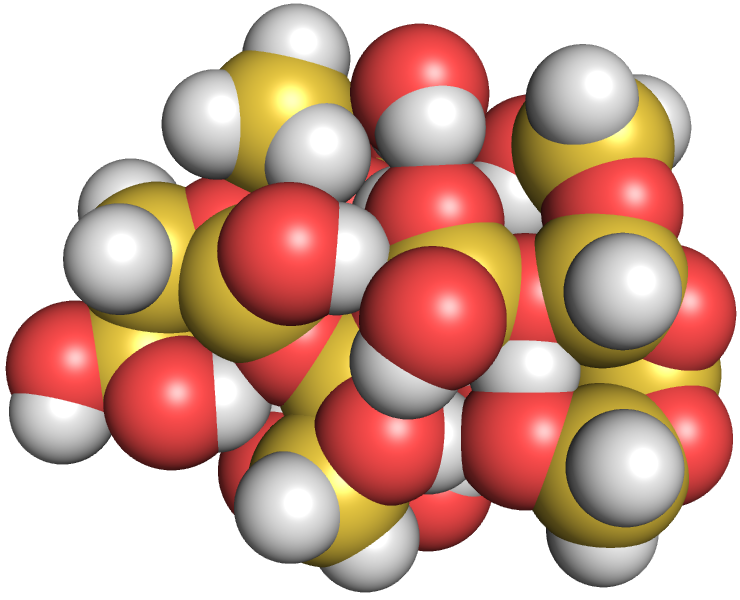
\includegraphics[width=\textwidth]{zhang_precursor_cluster}
    \subcaption{zhang: Cluster von Precursor-Molekülen}
  \end{subfigure}


  \caption[Cluster von Precursormolekülen]{Clusterbildung von Precursormolekülen bei 500K}
  \label{fig:precursorclusters}

\end{figure}
